%%%%% Single page layout:
%%%%% ----------------------------------------------------
\documentclass[12pt,a4paper,paper=a4,oneside,titlepage,pdftex]{scrartcl} 

%%% Additional useful packages
%%% ----------------------------------------------------------------
\usepackage{amsmath,amssymb,amsfonts}
\usepackage{algorithmic}
\usepackage{graphicx}
\usepackage{multirow}
\usepackage{array}
\usepackage{listings}                
\usepackage{subcaption}
\usepackage{float}
\usepackage[utf8]{inputenc}
\usepackage{booktabs}
\usepackage{pdfpages}
\usepackage{hyperref}
\usepackage{url}
\usepackage{color} %red, green, blue, yellow, cyan, magenta, black, white

%table caption on top
\usepackage{float}
\floatstyle{plaintop}
\restylefloat{table}

%custom command to rotate text
\newcommand*\rot{\rotatebox{90}}

\begin{document}
	
\pagenumbering{arabic}

\title{Project Report: Users' satisfaction about Dalarna University's Homepage}
\subtitle{ST3012 Data Collection}
\author{
	\bfseries\Large Authors: Péter Tempfli, Tobias Weiß\\
	\{v19pette, v18tobwe\}@du.se
	\\ \\
	
\includegraphics[]{figures/du-logo.jpg}\\
}

\maketitle
\tableofcontents
\newpage

\section{Abstract}
We write as very last thing
\vspace{10px}
\textbf{Keywords: foo bar}

\section{Introduction - Tobias}
Not long time ago, Dalarna University decided to update the website layout to cutting-edge web technologies. To set up a website is easy but who guarantees that the users are satisfied with it? With this project we help to increase the understanding of user needs and how well these needs are suited by the prevailing system.

\subsection{Research Question}
Users' satisfaction is a very broad topic and the scope has to be narrowed down carefully. A survey about general satisfaction would be doomed to fail. It either would be too big and comprehensive or too general and vague. Both would lead to missing and/or imprecise information. Therefore, this project focuses on functionality aspects of the "search personal" page. Following main questions were raised:
\begin{enumerate}
	\item If "find personal" is accessed, then the path is intuitive and quick?
	\item If "find personal" page is visited, then the required data is found quickly?
	\item If "find personal" page is visited, then a up-to-date front-end is displayed?
\end{enumerate}

In oder to answer these questions a survey among the website users is conducted.

\section{Methodology}
A qualitative survey \cite{sofaer1999qualitative} with quantified questions is suggested as functionality remains a subjective impression. For quantification a five-point Likert scale \cite{likert1932technique} is used. The scale is not directly visible to the subject as questions can be answered with sentences like "I fully agree", "I agree", etc. There is a discussion \cite{cummins2000we} whether five-point Likert scales are a sound method or not. This research sticks to it as more sophisticated methods \cite{chimi2009likert} seem unhandy and are not easily adaptable in the system, which is used for data collection.

\subsection{Research design}
A Google docs online form is chosen to conduct the research. It seems to be used in other educational context \cite{gehringer2010daily} but is not suggested in research beyond a Master thesis level. Dalarna University offers a survey tool which should be used instead in a real context.

\subsubsection{Population - Tobias}
The population are all human beings who have visited the Dalarna University website in the past and who will visit it in the future. One can estimate their number by analyzing server logs but still has to narrow down the time (visitors during the last month) and make certain assumptions.

\subsubsection{Sampling size - Tobias}
As no previous data is available, one has to assume the most conservative P value of $ P = 0.5 $. Furthermore, the standard values of 10\% for error level and 95\% for the confidence interval are assumed. Therefore, the sampling size is calculated as shown in equation \ref{eq:sampling-size}.

\begin{equation}
n = Z^2_\alpha \frac{P\dot(1-P)}{(\hat{p}-P)^2} = 1.96^2\frac{0.5\dot{(1-0.5)}}{0.1^2}=96 \text{ subjects}
\label{eq:sampling-size}
\end{equation}

\subsubsection{Data collection plan - Tobias}
As the survey is not carried out on the full sample but just on a few show cases, we send an E-Mail or WhatsApp message with link to the Google forms document and explanation to some of our classmates.
\\ \\
In reality, an implementation of sequential sampling as described by Fan et al. \cite{fan1962development} is suggested directly on the website. If users search a person e.g. the depicted binomial approach can be applied to show a overlay with an invitation link to the survey. Still, it remains questionable if the structure of respondents is representative and delivers an unbiased view as humans tend only to report unwanted results \cite{bergstrand1983bias}. Maybe incentives to answer the questionnaire have to be introduced.

\subsubsection{Statistical Indicators}
About the Statistical methods we apply. Here go the dummy tables

\subsubsection{Data Quality Assurance}
Why we use the DESAP checklist

\subsubsection{Data collection plan}
Why (only) a on line survey. Why on line?

%\begin{figure}[H]
%    \centering
%    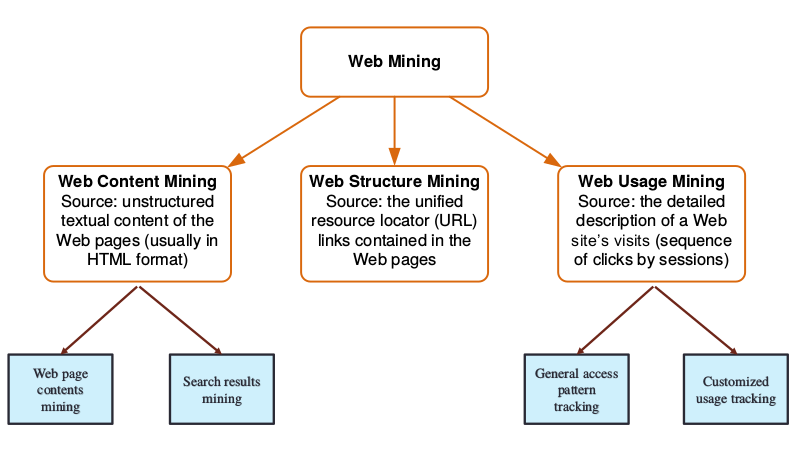
\includegraphics[width=0.7\textwidth]{figures/typed-of-webmining.png}
%    \caption{dummy}
%    \label{fig:XXX}
%\end{figure}

\subsubsection{Ethical considerations}
How do we store the data? What is the problem with Google forms. (Maybe write that in a real research we would use our own form/tool!)

\subsubsection{Legal considerations}
GDPR checkbox in the survery

\subsubsection{Analysis plan}
For the questions we use cross tables, to calculate absolute and relative frequencies as well as the $\chi^2$ coefficient. A dummy table is represented by table \ref{tab:dummy-crosstable}.

\begin{table}
	\centering
    \begin{tabular}{ | r || c | c | c | c | c || r |}
      \hline
        & \rot{I fully agree} & \rot{I agree}  & \rot{I mainly agree}  & \rot{I partly disagree}  & \rot{I disagree} & $\Sigma$ \\ \hline \hline
      pupil & 0 & 0 & 0 & 0 & 0 & 0 \\ \hline
      student from other institution & 0 & 0 & 0 & 0 & 0 & 0 \\ \hline
      researcher from other institution & 0 & 0 & 0 & 0 & 0 & 0 \\ \hline
      student @DU & 0 & 0 & 0 & 0 & 0 & 0 \\ \hline
      researcher/employee @DU & 0 & 0 & 0 & 0 & 0 & 0 \\ \hline
      other & 0 & 0 & 0 & 0 & 0 & 0 \\ \hline \hline
      $\Sigma$ & 0 & 0 & 0 & 0 & 0 & 0 \\ \hline
    \end{tabular}
  \caption{Dummy cross table for all questions}

  \label{tab:dummy-crosstable}
\end{table}


\section{Analysis}

\subsection{Pilot}

\subsection{Absolute and Relative Frequencies}

\subsection{(Co-)variances}

\subsection{Independence}

\section{Conclusion}

\section*{References}
\bibliographystyle{ieeetr}
\renewcommand\refname{\vskip -1cm}
\bibliography{ST3012_project_report_v19pette_v18tobwe}

\section*{Appendices}

\subsection*{Survey Guideline}
Information about the questions

\subsection*{Survey Questions}
Only absolute relevant questions

\subsection*{DESAP checklist}
Checklist can be found in the git folder

\end{document}
